\newcommand*{\eg}{e.g.\@\xspace}
\newcommand*{\ie}{i.e.\@\xspace}
\newcommand*{\cf}{cf.\@\xspace}
\newcommand{\amsbound}{\textsc{AMSBound}\xspace}
\newcommand{\adabound}{\textsc{AdaBound}\xspace}
\newcommand{\adam}{\textsc{Adam}\xspace}
\newcommand{\momentum}{\textsc{Momentum}\xspace}
\newcommand{\sgd}{\textsc{SGD}\xspace}
\newcommand{\rmsprop}{\textsc{RMSProp}\xspace}
\newcommand{\amsgrad}{\textsc{AMSGrad}\xspace}
\newcommand{\adadelta}{\textsc{Adadelta}\xspace}
\newcommand{\nag}{\textsc{NAG}\xspace}
\newcommand{\nadam}{\textsc{Nadam}\xspace}
\newcommand{\radam}{\textsc{Radam}\xspace}
\newcommand{\norm}[1]{\left\lVert#1\right\rVert}
\newcommand{\plus}{\raisebox{.4\height}{\scalebox{.6}{+}}}
\newcommand{\minus}{\raisebox{.4\height}{\scalebox{.8}{-}}}
\newcommand{\imagequadsize}{1cm}


\chapter{Domain Generalization} % Main chapter title
\label{DomainGeneralization} 

Machine learning systems often lack \emph{out-of-distribution generalization} which causes models to heavily rely on the distribution provided by the training data and as a result don't perform very well when presented with irregular qualities during testing. For example, this can be seen in application scenarios where intelligent systems don't generalize well across health centers if the training data was collected in a single hospital \citep{Castro_2020, AlBadawy2018, PeroneBBC19} or when self-driving cars struggle under alternative lighting or weather conditions \citep{DaiG18, VolkMBH019}. Often, properties which are falsely interpreted as part of the relevant feature set include backgrounds \citep{BeeryHP18}, textures \citep{GeirhosRMBWB19}, or racial biases \citep{StockC18}. Due to the prevalence of this task for the wide-spread deployment of machine learning systems in flexible environments, many researchers in the last decade tried to tackle this task with various approaches. In this chapter, we want to give a broad overview over the literature in \emph{domain generalization} and prepare the fundamentals for the following chapters. If you are already familiar with the field you can safely skip this part.

\section{Problem formulation}
\label{sec:domain_gen_problem}

\paragraph{Supervised Learning}
In supervised learning we are aiming to optimize the predictions $\mathbf{\hat{y}}$ for the values $\mathbf{y} \in \mathcal{Y}$ of a random variable $Y$, when presented with values $\mathbf{x} \in \mathcal{X}$ of a random variable $X$. These predictions are generated with a model predictor $f(\cdot;\boldsymbol{\theta}): \mathcal{X} \rightarrow \mathcal{Y}$ that is parameterized by parameters $\boldsymbol{\theta} \in \Theta$  and is assigning the predictions as $\mathbf{\hat{y}}=f(\cdot;\boldsymbol{\theta})$. To improve our predictions, we utilize a training dataset containing $n$ input-output pairs denoted as $D=\left\{\left(\mathbf{x}_{i}, \mathbf{y}_{i}\right)\right\}_{i=1}^{n}$ where each sample $(\mathbf{x}_i,\mathbf{y}_i)$ is ideally drawn identically and independently distributed (i.i.d.) from a single joint probability distribution $P(X,Y)$. By using a loss term $\mathcal{L} (\mathbf{\hat{y}};\mathbf{y}): \mathcal{Y} \times \mathcal{Y} \rightarrow \mathbb{R}^{+}$, which quantifies how different the prediction $\mathbf{\hat{y}}$ is from the ground truth $\mathbf{y}$, we would like to minimize the risk $R(f) = \mathbb{E}_{(\mathbf{x}, \mathbf{y}) \sim P}[\mathcal{L}(f(\mathbf{x}; \boldsymbol{\theta}), \mathbf{y})]$ of our model. Since we only have access to the distribution $P(X,Y)$ through a proxy in the form of the dataset $D$, we are instead minimizing the empirical risk $R_{\mathrm{emp}}(f)=\frac{1}{n} \sum_{i=1}^n \mathcal{L}\left(f\left(\mathbf{x}_{i};\boldsymbol{\theta}\right), \mathbf{y}_{i}\right)$ by adding up the loss terms of each sample. One common choice for this is the Cross-Entropy (CE) Loss which is shown in \Cref{eq:cross_entropy}.
\begin{equation}
\label{eq:cross_entropy}
    \mathcal{L}_\mathrm{ce}(\mathbf{y}, \mathbf{\hat{y}})=-\sum_{c=1}^{K} y_c \cdot \log \left(\hat{y}_c\right)
\end{equation}
Here, $\mathbf{y}$ is the one-hot vector representing the ground truth class, $\mathbf{\hat{y}}$ is the \emph{softmax} output of the model, and $y_i$, $\hat{y}_i$ are the $c$-th dimension of $\mathbf{y}$ and $\mathbf{\hat{y}}$.

The occurring minimization problem is then often solved through iterative gradient based optimization algorithms \eg \sgd{} \citep{Robbins1951} or \adam \citep{Kingma2015} which perform reasonably well for the non-convex, continuous loss surfaces produced by modern machine learning problems.

On top of that, the model predictor $f$ can be decomposed into two functions as $f=w \circ \phi$ where $\phi: \mathcal{X} \rightarrow \mathcal{Z}$ is an embedding into a feature space, hence sometimes called the feature extractor, and $w: \mathcal{Z} \rightarrow \mathcal{Y}$ which is sometimes called the classifier since it is a prediction from the feature space to the output space \citep{gulrajani2020search, MotiianPAD17}. This allows for a more concise mathematical notation.

\paragraph{Domain Generalization}
The problem of \emph{Domain generalization} (DG) builds on top of this framework, where now we have a set of training domains $\mathcal{S} = \left\{\mathcal{D}^{1}, \ldots, \mathcal{D}^{d_{\mathrm{tr}}}\right\}$ with $d \in\left\{1, \ldots, d_{\mathrm{tr}}\right\}$, where each $d$-th domain $\mathcal{D}^d$ has a dataset $D^{d}=\left\{\left(\mathbf{x}_{i}^{d}, \mathbf{y}_{i}^{d}\right)\right\}_{i=1}^{n_{d}}$ containing $n_d$ i.i.d. samples from individual distributions $P\left(X^{d}, Y^{d}\right)$. Here, $\mathbf{x}_i^d \in \mathbb{R}^{m}$ is the $i$-th sample for domain $\mathcal{D}^d$ representing a $m$-dimensional feature vector and $\mathbf{y}_i^d$ is the corresponding one-hot vector representing the ground truth class label. From these domains, we try to learn generic feature representations agnostic to domain changes to improve model performance \citep{seo2019learning}. Simply, we try to do \emph{out-of-distribution generalization} where our model aims to achieve good performance for an unseen test domain $d_\mathrm{te}$ sampled from the set of unseen domains $\mathcal{U} = \left\{\mathcal{D}^{1}, \ldots, \mathcal{D}^{d_{\mathrm{max}}}\right\}$ with $\mathcal{S} \cap \mathcal{U}=\emptyset$ based on statistical invariances across the observed training (source) and testing (target) domains \citep{gulrajani2020search, huang2020selfchallenging}. Hence, we try to minimize the expected target risk of our model as shown in \Cref{eq:domain_risk}.
\begin{equation}
\label{eq:domain_risk}
    R(f) = \mathbb{E}_{(\mathbf{x}^{d_{\mathrm{te}}}, y^{d_{\mathrm{te}}}) \sim P}[\mathcal{L}(f(\mathbf{x}^{d_{\mathrm{te}}}; \boldsymbol{\theta}), \mathbf{y}^{d_{\mathrm{te}}})]
\end{equation}
One simple approach is to apply the empirical risk minimization seen previously to the domain generalization task as shown in \Cref{eq:domain_risk_emp}, where we hope that minimizing the empirical risk over all source domains in $\mathcal{S}$ achieves good generalization to the target domain.
\begin{equation}
\label{eq:domain_risk_emp}
    R_\mathrm{emp}(f) = \frac{1}{d_\mathrm{tr}} \sum_{d=1}^{d_\mathrm{tr}} \frac{1}{n_d} \sum_{i=1}^{n_d} \mathcal{L}(f(\mathbf{x}_i^{d}; \boldsymbol{\theta}), \mathbf{y}_i^{d})
\end{equation}
The difference of this approach when compared to ordinary supervised learning is summarized on a high-level in \Cref{tab:learning_setups}. It may be helpful to think about a meta-distribution $\mathfrak{D}$ (real-world) generating source domains $\mathcal{D}^d_\mathcal{S}$ and unseen testing domains $\mathcal{D}^d_\mathcal{U}$ as shown in \Cref{fig:meta_domain}.
\begin{figure}[htbp]
    \centering
    \begin{tikzpicture}[
            > = stealth, % arrow head style
            shorten > = 1pt, % don't touch arrow head to node
            auto,
            node distance = 3cm, % distance between nodes
            semithick % line style
        ]
    \tikzstyle{every state}=[
            draw = black,
            thick,
            fill = white,
            minimum size = 1cm
        ]

        \node[state] (meta) at (0,0) {\Large{$\mathfrak{D}$}};
        \node[state] (d1) at (-3,-2) {$\mathcal{D}^1_\mathcal{S}$};
        \node[state] (d2) at (-1,-2) {$\mathcal{D}^{d_\mathrm{tr}}_\mathcal{S}$};
        \node[state] (d3) at (1,-2) {$\mathcal{D}^1_\mathcal{U}$};
        \node[state] (d4) at (3,-2) {$\mathcal{D}^{d_\mathrm{te}}_\mathcal{U}$};

        \path[->] (meta) edge node {} (d1);
        \path[->] (meta) edge node {} (d2);
        \path[->] (meta) edge node {} (d3);
        \path[->] (meta) edge node {} (d4);
        \path (d1) -- node[auto=false]{\ldots} (d2);
        \path (d3) -- node[auto=false]{\ldots} (d4);
    \end{tikzpicture}
    \caption[Meta-distribution $\mathfrak{D}$ generating source and unseen domains]{Meta-distribution $\mathfrak{D}$ generating source and unseen domains adapted from: \citep{albuquerque2019generalizing}}
    \label{fig:meta_domain}
\end{figure}

\begin{table}[t]
    \centering
    \begin{tabular}{lll}
    \toprule
    \textbf{Setup} & \textbf{Training inputs}  & \textbf{Testing inputs} \\
    \midrule
        Generative learning & $U^1$ & $\emptyset$ \\ 
        Unsupervised learning & $U^1$ & $U^1$  \\ 
        Supervised learning & $L^1$ & $U^1$ \\ 
        Semi-supervised learning & $L^{1}, U^{1}$ & $U^1$ \\ 
        Multitask learning & $L^{1}, \ldots, L^{d_{\mathrm{tr}}}$ & $U^{1}, \ldots, U^{d_{\mathrm{tr}}}$ \\ 
        Continual (lifelong) learning & $L^{1}, \ldots, L^{\infty}$ & $U^{1}, \ldots, U^{\infty}$ \\ 
        Domain adaption & $L^{1}, \ldots, L^{d_{\mathrm{tr}}}, U^{d_{\mathrm{tr}}+1}$ & $U^{d_{\mathrm{tr}}+1}$ \\ 
        Transfer learning & $U^{1}, \ldots, U^{d_{\mathrm{tr}}}, L^{d_{\mathrm{tr}}+1}$ & $U^{d_{\mathrm{tr}}+1}$ \\ 
        \textbf{Domain generalization} & $L^{1}, \ldots, L^{d_{\mathrm{tr}}}$ & $U^{d_{\mathrm{tr}}+1}$ \\ 
    \bottomrule
    \end{tabular}
    \caption[Differences in learning setups]{Differences in learning setups adapted from \citet{gulrajani2020search}. For each domain $d$ the labeled and unlabeled distributions are denoted as $L^d$ and $U^d$ respectively.}
    \label{tab:learning_setups}
\end{table}

\paragraph{Homogeneous and Heterogeneous}
Sometimes, domain generalization is also divided into \emph{homogeneous} and \emph{heterogeneous} subtasks. In homogeneous DG we assume that all domains share the same label space $\mathcal{Y}^{d_1} = \mathcal{Y}^{d_2} = \mathcal{Y}^{d_\mathrm{te}}$, $\forall d_1, d_2 \in \left\{1, \ldots, d_{\mathrm{tr}}\right\}$. On the contrary, the more challenging heterogeneous DG allows for different label spaces $\mathcal{Y}^{d_1} \neq \mathcal{Y}^{d_2} \neq \mathcal{Y}^{d_\mathrm{te}}$ which can even be completely disjoint \citep{LiZYLSH19}. For this work we assume the homogeneous setting.

\paragraph{Single- and Multi-Source}
There exist subtle differences within this task which are called \emph{single-} or \emph{multi-source domain generalization}. While multi-source domain generalization refers to the standard setting we have just outlined, single-source domain generalization is a more generic formulation \citep{zunino2020explainable}. Instead of relying on multiple training domains to learn models which generalize better, single-source domain generalization aims at learning these representations with access to only one source distribution. Hence, our training domains are restricted to $\mathcal{S} = \left\{\mathcal{D}^{1}\right\}$, described by one dataset $D^1=\left\{\left(\mathbf{x}^1_{i}, \mathbf{y}^1_{i}\right)\right\}_{i=1}^{n_{1}}$ and modeling a single source distribution $P\left(X^1, Y^1\right)$. This is different from the ordinary supervised learning setup since we want to analyze the performance of the model under a clear domain-shift (\ie out-of-distribution generalization). Note, that strong regularization methods will also perform well on this scenario. These cross-overs and related techniques are described in the following section.

\section{Related concepts and their differences}

Members of the causality community might know the task of domain generalization under the term \emph{learning from multiple environments} \citep{arjovsky2019invariant, gulrajani2020search, PetBuhMei15}. While these two concepts refer to the same task, there exist quite a few related techniques which we want to highlight here and distinguish in their scope. In particular, we focus on ``Generic neural network regularization'' and ``Domain Adaption'' since these are very closely related and sometimes hard to distinguish if at all. The overview in \Cref{tab:learning_setups}, however, includes even more learning setups to properly position this concept into the machine learning landscape.

\subsection{Generic Neural Network Regularization}

In theory, generic model regularization which aims to prevent neural networks from overfitting on the source domain, could also improve the domain generalization performance \citep{huang2020selfchallenging}. As such, methods like dropout \citep{SrivastavaHKSS14}, early stopping \citep{CaruanaLG00}, or weight decay \citep{NowlanH92} can have a positive effect on this task when deployed properly. Apart from regular dropout, where we randomly disable neurons in the training phase to stop them from co-adapting too much, a few alternative methods exist. These include dropping random  patches of input images (Cutout \& HaS) \citep{devries2017improved, SinghL17} or channels of the feature map (SpatialDropout) \citep{TompsonGJLB15}, dropping contiguous regions of the feature maps (DropBlock) \citep{GhiasiLL18}, dropping features of high activations across feature maps and channels (MaxDrop) \citep{ParkK16}, or generalizing the traditional dropout of single units to entire layers during training (DropPath) \citep{LarssonMS17}. There even exist methods like curriculum dropout \citep{MorerioCVVM17} which deploy scheduling for the dropout probability and therefore softly increase the amount of units to be suppressed layerwise during training. 

Generally, deploying some of these methods when aiming for out-of-distribution generalization can be a good idea and should definitely be considered for the task of domain generalization.


\subsection{Domain Adaption}

\emph{Domain adaption} (DA) is often mentioned as a closely related task in domain generalization literature \citep{MotiianPAD17, VolpiM19, QiaoZP20}. When compared, domain adaption has additional access to an unlabeled dataset from the target domain \citep{mancini2020, Csurka17}. Formally, aside from the set of source domains $\mathcal{S}$ and the domain datasets $D^d$, as outline in \Cref{sec:domain_gen_problem}, we have access to target samples $\mathcal{T} = \left\{\mathbf{x}_{1}^{d_\mathrm{te}},\dots,\mathbf{x}_{n_{d_{\mathrm{te}}}}^{d_\mathrm{te}}\right\}$ that are from the target domain $\mathbf{x}_j^{d_{ \mathrm{te}}} \sim P(X^{d_{ \mathrm{te}}},Y^{d_{ \mathrm{te}}})$ but their labels remain unknown in training since we want to predict them during testing. As a result, domain generalization is considered to be the harder problem of the two. This difference is also shown in \Cref{tab:learning_setups}.

Earlier methods in this space deploy hand-crafted features to reduce the difference between the source and the target domains \citep{ManciniPBC018}. Like that, \emph{instance-based methods} try to re-weight source samples according to target similarity \citep{GongGS13, HuangSGBS06, YamadaSR12} or \emph{feature-based methods} try to learn a common subspace \citep{FernandoHST13, GongSSG12, LongD0SGY13, BaktashmotlaghHLS13}. More recent works focus on \emph{deep domain adaption} based on deep architectures where domain invariant features are learned utilizing supervised neural networks \citep{BousmalisTSKE16, CarlucciPCRB17, GaninL15, GhifaryKZBL16}, autoencoders \citep{ZengOWW14}, or generative adversarial networks (GANs) \citep{BousmalisSDEK17, ShrivastavaPTSW17, TzengHSD17}. These deep neural network based architectures significantly outperform the approaches for hand-crafted features \citep{ManciniPBC018}.

Even though domain adaptation and domain generalization both try to reducing dataset bias, they are not compatible to each other \citep{GhifaryBKZ17}. Hence, domain adaptation methods often cannot be directly used for domain generalization or vice versa \citep{GhifaryBKZ17}. For this work, we don't rely on the simplifying assumptions of domain adaption, but instead tackle the more challenging task of domain generalization.

\section{Previous Works}

No idea where to fit these yet: 

2018: 
\citep{NiuLXC18}

2019: 
\citep{VolpiM19} 
\citep{yao2019adversarial}
\citep{arjovsky2019invariant}
\citep{seo2019learning}

2020: 
\citep{QiaoZP20}
\citep{bellot2020generalization}
\citep{jin2020feature}
\citep{somavarapu2020frustratingly}
\citep{deng2020representation}
\citep{mahajan2020domain}
\citep{wang2020learning}
\citep{du2020learning}
\citep{huang2020selfchallenging}
\citep{zhou2020learning}
\citep{Jia_2020_CVPR_SSDG}
\citep{piratla2020efficient}
\citep{RyuK0L20}
\citep{zunino2020explainable}






Since literature in the domain generalization space is very broad, we utilized Appendix A in \citet{gulrajani2020search} for an overview and individually added additional works and information where necessary.  

\subsection{Learning invariant features}

Some of the earliest works on learning invariant features were \emph{kernel methods} applied by \citet{MuandetBS13}  where they look for a feature transformation that minimizes the across-domain dissimilarity between transformed feature distributions while preserving the functional relationship between original features and targets. In recent years, there have been approaches following a similar kernel based approach \citep{LiGTLT18, LiTGLLZT18}, sometimes while maximizing class separability \citep{Hu0CC19, GhifaryBKZ17}. As an early method, \citet{FangXR13} introduce Unbiased Metric Learning (UML) with a SVM metric that enforces the neighborhood of samples to contain samples with the same class label but from other training domains.

After that, \citet{GaninUAGLLML16} introduced Domain Adversarial Neural Networks (DANNs) utilizing neural network architectures to learn domain-invariant feature representations by adding a gradient reversal layer. Recently, their approach got extended to support statistical dependence between domains and class labels \citep{AkuzawaIM19} or considering one-versus-all adversaries to minimize pairwise divergences between source distributions \citep{albuquerque2019generalizing}. \citet{MotiianPAD17} use a siamese architecture to learn a feature transformation which tries to achieve semantical alignment of visual domains while maximally separating them. Other methods are also matching the feature covariance across source domains \citep{RahmanFBS20}.

\citet{MatsuuraH20} use clustering techniques to split single-source domain generalization into different domains and then train a domain-invariant feature extractor via adversarial
learning. 

\citet{LiPWK18} deploy adversarial autoencoders with maximum mean discrepancy (MMD) \citep{GrettonBRSS12} to align the source distributions, \ie for distributions $P$, $Q$ and a feature map $\varphi: \mathcal{X} \rightarrow \mathcal{H}$ where $\mathcal{H}$ is a reproducing kernel Hilbert space (RKHS) this measure is defined as \Cref{eq:mmd}.
\begin{equation}
\label{eq:mmd}
    \operatorname{MMD}(P, Q)=\left\|\mathbb{E}_{X \sim P}[\varphi(X)]-\mathbb{E}_{Y \sim Q}[\varphi(Y)]\right\|_{\mathcal{H}}
\end{equation}
\citet{ilse2019diva} extend the variational autoencoder \citep{KingmaW13} by introducing latent representations for domains $\mathcal{Z}_d$, classes $\mathcal{Z}_y$ and residual variations $\mathcal{Z}_x$. \citet{LiZYLSH19} use episodic training \ie they train a domain agnostic feature extractor $\phi$ and classifier $w$ by mismatching them with an equivalent trained on a specific domain in combinations $(\phi^{d_1}, w, \mathbf{x}^{d_2}_i)$ and $(\phi, w^{d_1}, \mathbf{x}^{d_2}_i)$ and letting them predict data outside of the trained domain $d_1 \neq d_2$. \citet{li2020sequential} use a lifelong sequential learning strategy.

\subsection{Model ensembling}

Some methods try to associate model parameters with each of the training domains and combine them with shared parameters in a meaningful matter to improve generalization to the test domain. Often, the amount of models in these type of architectures grow linearly with the number of source domains. The first work to pose the problem of domain generalization and analyze it was \citet{BlanchardLS11}. In there, they use classifiers for each sample $\mathbf{x}^d$  denoted as $f(\mathbf{x}^d,\mu^d)$ where $\mu^d$ corresponds to a kernel mean embedding \citep{MuandetFSS17}. For theoretical analysis on such methods please see \citet{an2019generalization} and \citet{blanchard2017domain}. Later on, \citet{KhoslaZMET12} combine global weights $w$ with local domain biases $\Delta^d$ to learn one max-margin linear classifier (SVM) per domain as $w^d = w + \Delta^d$ and finally combine them, which has recently been extended to neural network settings by adding an additional dimension describing the training domains to the parameter tensors \citep{LiYSH17}. \citet{GhifaryKZB15} propose a Multi-task Autoencoder (MTAE) with shared parameters to the hidden state and domain-specific parameters for each of the training domains. Further, \citet{ManciniBCR18} use domain-specific batch-normalization \citep{IoffeS15} layers and then linearly combine them using a softmax domain classifier. Other works linearly combine domain-specific predictors \citep{ManciniBC018}, or use more elaborate aggregation strategies to combine these \citep{DInnocenteC18}. \citet{DingF18} use multiple
domain-specific deep neural networks with a structured low-rank constraint and a domain-invariant deep neural network to generalize to the target domain. There have also been works which assign weights to minibatches depending on their respective error to the training distributions \citep{HuNSS18, sagawa2019distributionally}.


\subsection{Meta-learning}
 \citet{FinnAL17} propose a Model-Agnostic Meta-Learning (MAML) algorithm which is able to quickly learn new tasks. \citet{LiYSH18} adapt this algorithm for domain generalization such that we can quickly adapt to new domains by utilizing the meta-optimization objective which ensures that steps to improve training domain performance should also improve testing domain performance. Both approaches are not bound to a specific architecture and can therefore be deployed for a wide variety of learning tasks. These approaches recently got extended by two regularizers that encourage general knowledge about inter-class relationships and domain-independent class-specific cohesion \citep{DouCKG19}, to instances of domain generalization where the label space varies from domain to domain \citep{LiYZH19}, or meta-learning a regularizer which encourages across-domain performance \citep{BalajiSC18}.

\subsection{Data Augmentation}
\emph{Data Augmentation} remains a competitive method for generalizing to unseen domains \citep{zhang2019unseen}. However, to deploy an efficient procedure for that, human experts need to consider the data at hand to develop a useful routine \citep{gulrajani2020search}. Several works have used the \textsc{mixup} \citep{ZhangCDL18} algorithm as a method to merge samples from different domains \citep{XuZNLWTZ20, yan2020improve, WangLK20, mancini2020}. Other works have also tried removing textural information from images \citep{WangHLX19} or shifting it more towards shapes \citep{nam2019reducing, asadi2019shape}. \citet{CarlucciDBCT19} used jigsaw puzzles of image patches as a classification task to show that this improves domain generalization while \citet{VolpiNSDMS18} demonstrate that adversarial data augmentation on a single domain is sufficient. Several methods also utilize GANs to augment the available training data  \citep{RahmanFBS19, ZhouYHX20, ShankarPCCJS18}. 

\section{Common Datasets}

\subsection{Rotated MNIST}
The rotated MNIST (RMNIST) dataset \citep{GhifaryKZB15} is a variation of the original MNIST dataset \citep{lecun-mnisthandwrittendigit-2010} where each digit got rotated by degrees $\{0, 15, 30, 45, 60, 75\}$. Each rotation angle represents one domain as shown in \Cref{tab:common_examples} for classes ``2'' and ``4''. The overall dataset in \citet{gulrajani2020search} includes \num{70000} images from $10$ homogeneous classes ($0-9$) each with dimension $1\times28\times28$.

\begin{table}[htbp]
    \centering
    \begin{tabularx}{\textwidth}{lcYYYYYY}
    \toprule
    \textbf{Dataset}  & \textbf{Reference} & $\mathcal{D}^1$   &  $\mathcal{D}^2$ & $\mathcal{D}^3$ & $\mathcal{D}^4$ & $\mathcal{D}^5$ & $\mathcal{D}^6$ \\
    \midrule
       \multirow{7}{*}{\textbf{Rotated MNIST}}  & \multirow{7}{*}{\textbf{\citep{GhifaryKZB15}}} & $0^\circ$ & $15^\circ$ & $30^\circ$ & $45^\circ$ & $60^\circ$ & $75^\circ$ \\
       & & 
\includegraphics[height=\imagequadsize, width=\imagequadsize]{Figures/Chapter2/RMNIST/RotatedMNIST_env00_2_idx470_class2.png} &  
\includegraphics[height=\imagequadsize, width=\imagequadsize]{Figures/Chapter2/RMNIST/RotatedMNIST_env115_6_idx8084_class2.png} &  
\includegraphics[height=\imagequadsize, width=\imagequadsize]{Figures/Chapter2/RMNIST/RotatedMNIST_env230_23_idx3711_class2.png} & 
\includegraphics[height=\imagequadsize, width=\imagequadsize]{Figures/Chapter2/RMNIST/RotatedMNIST_env345_9_idx11212_class2.png} &  
\includegraphics[height=\imagequadsize, width=\imagequadsize]{Figures/Chapter2/RMNIST/RotatedMNIST_env460_11_idx7785_class2.png} & 
       
\includegraphics[height=\imagequadsize, width=\imagequadsize]{Figures/Chapter2/RMNIST/RotatedMNIST_env575_27_idx3863_class2.png} \\
        & & 
\includegraphics[height=\imagequadsize, width=\imagequadsize]{Figures/Chapter2/RMNIST/RotatedMNIST_env00_19_idx5269_class4.png} &
\includegraphics[height=\imagequadsize, width=\imagequadsize]{Figures/Chapter2/RMNIST/RotatedMNIST_env115_8_idx7608_class4.png} & 
\includegraphics[height=\imagequadsize, width=\imagequadsize]{Figures/Chapter2/RMNIST/RotatedMNIST_env230_18_idx2042_class4.png} & 
\includegraphics[height=\imagequadsize, width=\imagequadsize]{Figures/Chapter2/RMNIST/RotatedMNIST_env345_7_idx6290_class4.png} & 
\includegraphics[height=\imagequadsize, width=\imagequadsize]{Figures/Chapter2/RMNIST/RotatedMNIST_env460_6_idx1791_class4.png} &
       
\includegraphics[height=\imagequadsize, width=\imagequadsize]{Figures/Chapter2/RMNIST/RotatedMNIST_env575_14_idx11054_class4.png} \\
       \addlinespace
       %%
       \multirow{7}{*}{\textbf{DomainNet}} &  \multirow{7}{*}{\textbf{\citep{PengBXHSW19}}} & Clipart & Graphic & Painting & Draw & Photo & Sketch \\
       & & 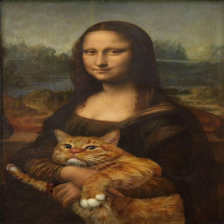
\includegraphics[height=\imagequadsize, width=\imagequadsize]{Figures/Chapter2/DomainNet/DomainNet_env0clipart_4_idx283_class2.png} & 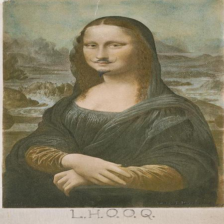
\includegraphics[height=\imagequadsize, width=\imagequadsize]{Figures/Chapter2/DomainNet/DomainNet_env1infograph_8_idx378_class2.png} & 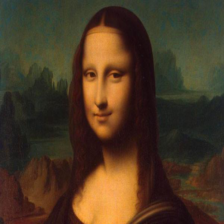
\includegraphics[height=\imagequadsize, width=\imagequadsize]{Figures/Chapter2/DomainNet/DomainNet_env2painting_41_idx507_class2.png} &  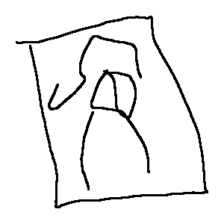
\includegraphics[height=\imagequadsize, width=\imagequadsize]{Figures/Chapter2/DomainNet/DomainNet_env3quickdraw_30_idx1326_class2.png} &  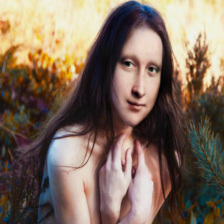
\includegraphics[height=\imagequadsize, width=\imagequadsize]{Figures/Chapter2/DomainNet/DomainNet_env4real_9_idx1117_class2.png} &  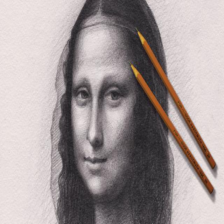
\includegraphics[height=\imagequadsize, width=\imagequadsize]{Figures/Chapter2/DomainNet/DomainNet_env5sketch_28_idx421_class2.png} \\
       &  & 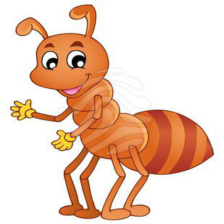
\includegraphics[height=\imagequadsize, width=\imagequadsize]{Figures/Chapter2/DomainNet/DomainNet_env0clipart_1_idx1098_class9.png} & 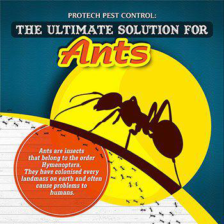
\includegraphics[height=\imagequadsize, width=\imagequadsize]{Figures/Chapter2/DomainNet/DomainNet_env1infograph_39_idx689_class9.png} & 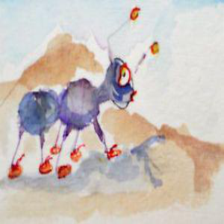
\includegraphics[height=\imagequadsize, width=\imagequadsize]{Figures/Chapter2/DomainNet/DomainNet_env2painting_25_idx2262_class9.png} & 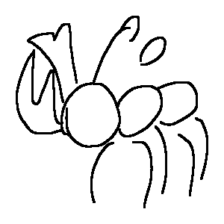
\includegraphics[height=\imagequadsize, width=\imagequadsize]{Figures/Chapter2/DomainNet/DomainNet_env3quickdraw_7_idx4907_class9.png} & 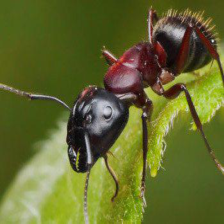
\includegraphics[height=\imagequadsize, width=\imagequadsize]{Figures/Chapter2/DomainNet/DomainNet_env4real_34_idx3532_class9.png} & 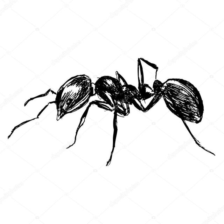
\includegraphics[height=\imagequadsize, width=\imagequadsize]{Figures/Chapter2/DomainNet/DomainNet_env5sketch_0_idx1772_class9.png} \\
       \addlinespace
       %%
       \multirow{7}{*}{\textbf{Office-Home}} & \multirow{7}{*}{\textbf{\citep{VenkateswaraECP17}}} & Art & Clipart & Product & Real & & \\
       & & 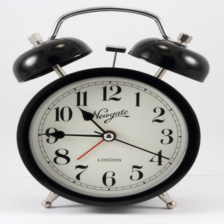
\includegraphics[height=\imagequadsize, width=\imagequadsize]{Figures/Chapter2/OfficeHome/OfficeHome_env0Art_1_idx61_class0.png} & 
\includegraphics[height=\imagequadsize, width=\imagequadsize]{Figures/Chapter2/OfficeHome/OfficeHome_env1Clipart_5_idx24_class0.png} & 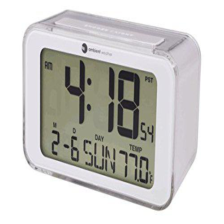
\includegraphics[height=\imagequadsize, width=\imagequadsize]{Figures/Chapter2/OfficeHome/OfficeHome_env2Product_14_idx67_class0.png} & 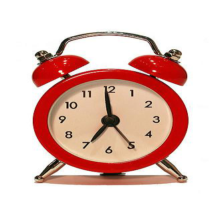
\includegraphics[height=\imagequadsize, width=\imagequadsize]{Figures/Chapter2/OfficeHome/OfficeHome_env3Real World_44_idx13_class0.png} & & \\
        & & 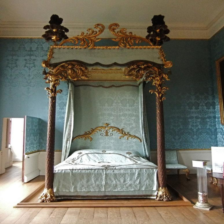
\includegraphics[height=\imagequadsize, width=\imagequadsize]{Figures/Chapter2/OfficeHome/OfficeHome_env0Art_18_idx176_class3.png} & 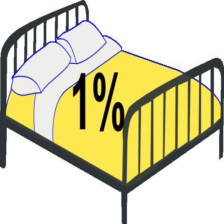
\includegraphics[height=\imagequadsize, width=\imagequadsize]{Figures/Chapter2/OfficeHome/OfficeHome_env1Clipart_12_idx199_class3.png} & 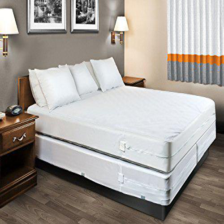
\includegraphics[height=\imagequadsize, width=\imagequadsize]{Figures/Chapter2/OfficeHome/OfficeHome_env2Product_19_idx261_class3.png} & 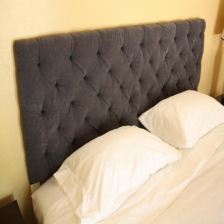
\includegraphics[height=\imagequadsize, width=\imagequadsize]{Figures/Chapter2/OfficeHome/OfficeHome_env3Real World_20_idx300_class3.png} & & \\
        \addlinespace
        %%
       \multirow{7}{*}{\textbf{VLCS}} & \multirow{7}{*}{\textbf{\citep{EveringhamGWWZ10, RussellTMF08, Griffin2007Caltech256OC, ChoiLTW10}}} & V & L & C & S & & \\ 
       & & 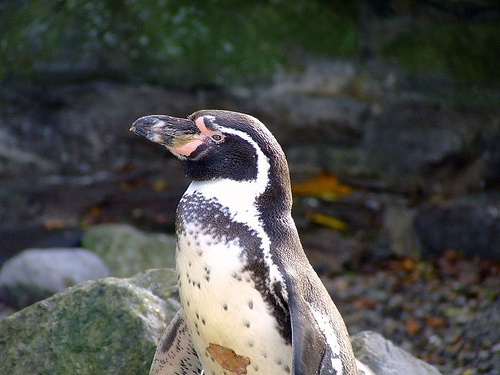
\includegraphics[height=\imagequadsize, width=\imagequadsize]{Figures/Chapter2/VLCS/voc_bird.jpg}  &  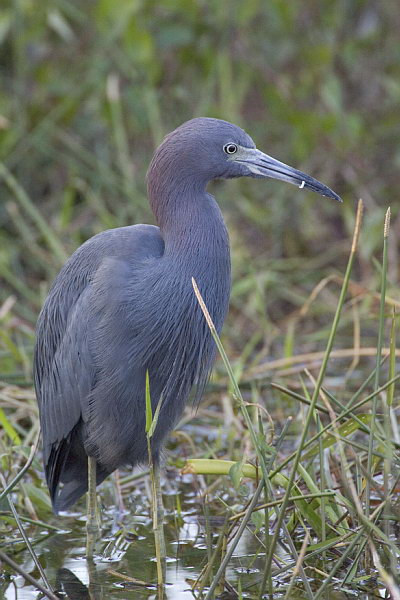
\includegraphics[height=\imagequadsize, width=\imagequadsize]{Figures/Chapter2/VLCS/labelme_bird.jpg} & 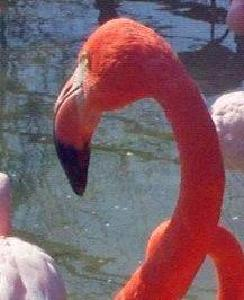
\includegraphics[height=\imagequadsize, width=\imagequadsize]{Figures/Chapter2/VLCS/caltech_bird.jpg} & 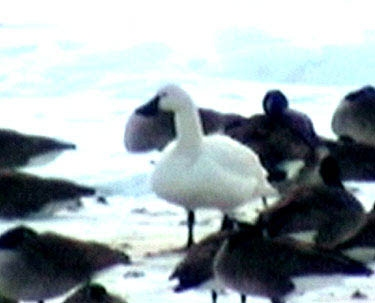
\includegraphics[height=\imagequadsize, width=\imagequadsize]{Figures/Chapter2/VLCS/sun_bird.jpg} & & \\
       & & 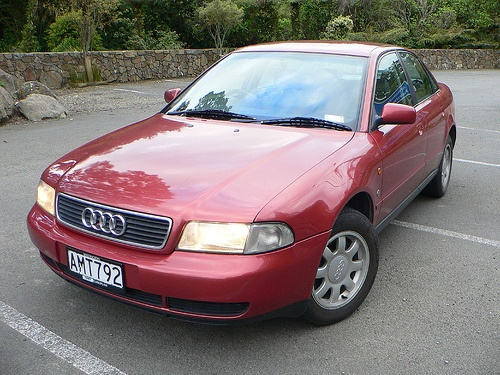
\includegraphics[height=\imagequadsize, width=\imagequadsize]{Figures/Chapter2/VLCS/voc_car.jpg} & 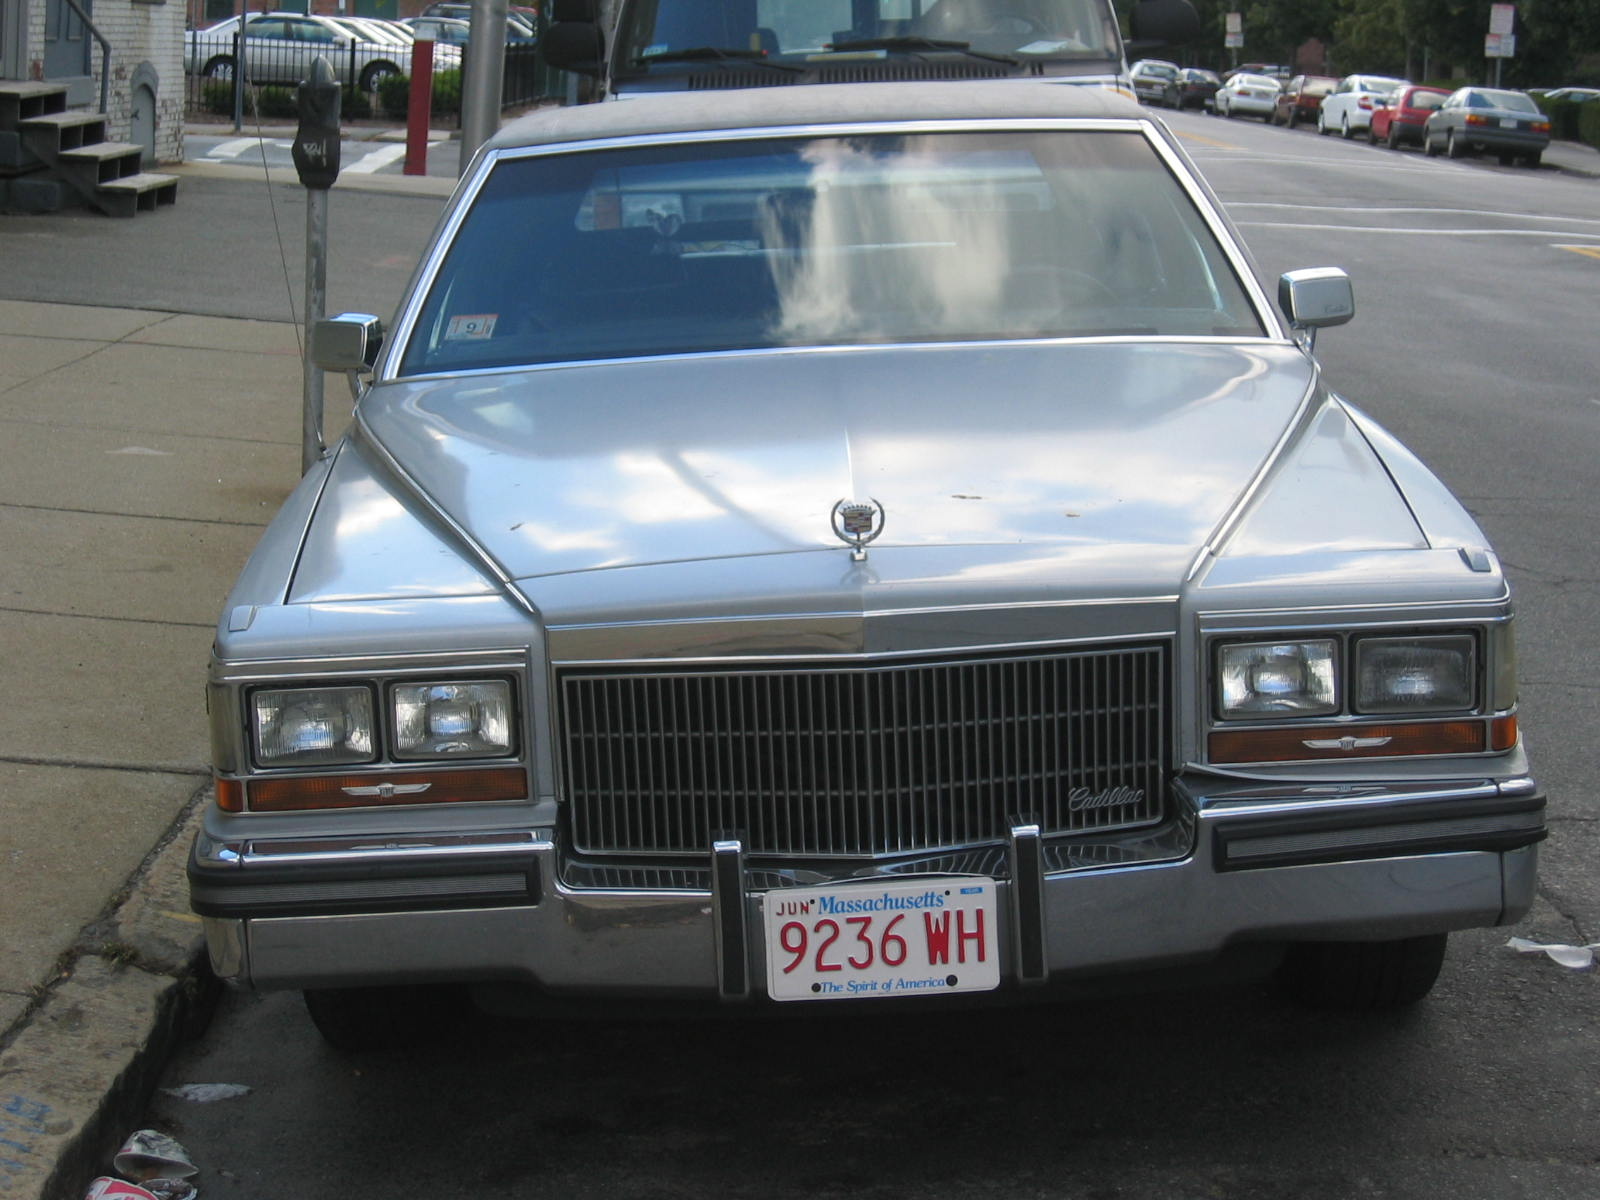
\includegraphics[height=\imagequadsize, width=\imagequadsize]{Figures/Chapter2/VLCS/labelme_car.jpg} & 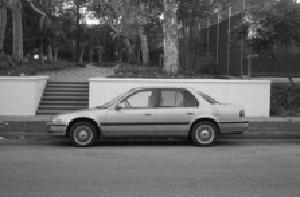
\includegraphics[height=\imagequadsize, width=\imagequadsize]{Figures/Chapter2/VLCS/caltech_car.jpg} & 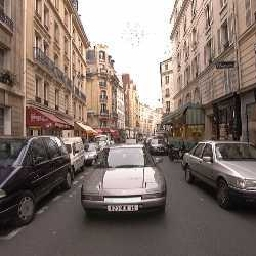
\includegraphics[height=\imagequadsize, width=\imagequadsize]{Figures/Chapter2/VLCS/sun_car.jpg} & & \\
       \addlinespace
       %%
       \multirow{7}{*}{\textbf{Terra Incognita}} & \multirow{7}{*}{\textbf{\citep{BeeryHP18}}} & L100 & L38 & L43 & L46 & & \\ 
       & & 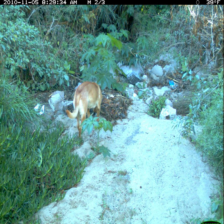
\includegraphics[height=\imagequadsize, width=\imagequadsize]{Figures/Chapter2/TerraIncognita/TerraIncognita_env0location_100_22_idx685_class4.png} &  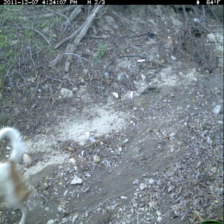
\includegraphics[height=\imagequadsize, width=\imagequadsize]{Figures/Chapter2/TerraIncognita/TerraIncognita_env1location_38_5_idx2429_class4.png} &
       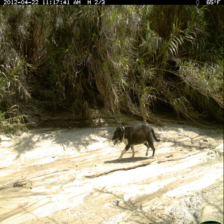
\includegraphics[height=\imagequadsize, width=\imagequadsize]{Figures/Chapter2/TerraIncognita/TerraIncognita_env2location_43_45_idx2058_class4.png} &  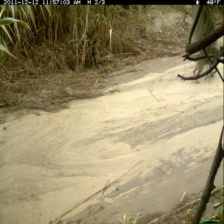
\includegraphics[height=\imagequadsize, width=\imagequadsize]{Figures/Chapter2/TerraIncognita/TerraIncognita_env3location_46_6_idx2012_class4.png} & & \\
       & & 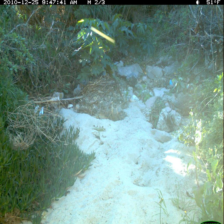
\includegraphics[height=\imagequadsize, width=\imagequadsize]{Figures/Chapter2/TerraIncognita/TerraIncognita_env0location_100_0_idx823_class5.png} & 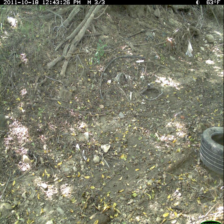
\includegraphics[height=\imagequadsize, width=\imagequadsize]{Figures/Chapter2/TerraIncognita/TerraIncognita_env1location_38_35_idx2747_class5.png} & 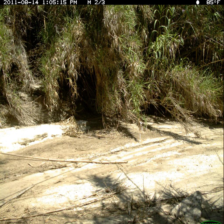
\includegraphics[height=\imagequadsize, width=\imagequadsize]{Figures/Chapter2/TerraIncognita/TerraIncognita_env2location_43_38_idx2211_class5.png} & 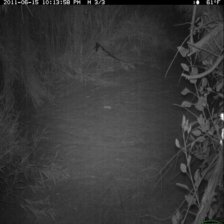
\includegraphics[height=\imagequadsize, width=\imagequadsize]{Figures/Chapter2/TerraIncognita/TerraIncognita_env3location_46_37_idx2142_class5.png} & & \\
       \addlinespace
       %%
       \multirow{7}{*}{\textbf{PACS}} & \multirow{7}{*}{\textbf{\citep{LiYSH17}}}  & Art & Cartoon & Photo & Sketch & & \\
       & & 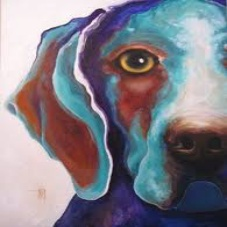
\includegraphics[height=\imagequadsize, width=\imagequadsize]{Figures/Chapter2/PACS/dog_1.jpg} &  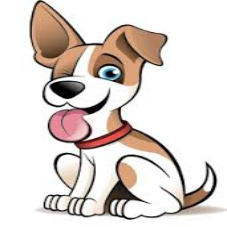
\includegraphics[height=\imagequadsize, width=\imagequadsize]{Figures/Chapter2/PACS/dog_2.jpg} &  \includegraphics[height=\imagequadsize, width=\imagequadsize]{Figures/Chapter2/PACS/dog_3.jpg} &  \includegraphics[height=\imagequadsize, width=\imagequadsize]{Figures/Chapter2/PACS/dog_4.png} & & \\
       & & \includegraphics[height=\imagequadsize, width=\imagequadsize]{Figures/Chapter2/PACS/elephant_1.jpg} & \includegraphics[height=\imagequadsize, width=\imagequadsize]{Figures/Chapter2/PACS/elephant_2.jpg} & \includegraphics[height=\imagequadsize, width=\imagequadsize]{Figures/Chapter2/PACS/elephant_3.jpg} & \includegraphics[height=\imagequadsize, width=\imagequadsize]{Figures/Chapter2/PACS/elephant_4.png} & & \\
       \addlinespace
       %%
       \multirow{7}{*}{\textbf{Colored MNIST}} & \multirow{7}{*}{\textbf{\citep{arjovsky2019invariant}}} & $\plus90\%$ & $\plus80\%$ & $\minus90\%$ & & & \\
       & & \includegraphics[height=\imagequadsize, width=\imagequadsize]{Figures/Chapter2/CMNIST/ColoredMNIST_env00.1_18_idx12999_class0.png} &  \includegraphics[height=\imagequadsize, width=\imagequadsize]{Figures/Chapter2/CMNIST/ColoredMNIST_env10.2_11_idx22249_class0.png} & \includegraphics[height=\imagequadsize, width=\imagequadsize]{Figures/Chapter2/CMNIST/ColoredMNIST_env20.9_1_idx13997_class0.png} & & & \\
        & & \includegraphics[height=\imagequadsize, width=\imagequadsize]{Figures/Chapter2/CMNIST/ColoredMNIST_env00.1_8_idx9692_class1.png} & \includegraphics[height=\imagequadsize, width=\imagequadsize]{Figures/Chapter2/CMNIST/ColoredMNIST_env10.2_5_idx15365_class1.png} & \includegraphics[height=\imagequadsize, width=\imagequadsize]{Figures/Chapter2/CMNIST/ColoredMNIST_env20.9_9_idx7793_class1.png}  & & & \\
        \addlinespace
    \bottomrule
    \end{tabularx}
    \caption{Samples for two different classes across domains for popular datasets}
    \label{tab:common_examples}
\end{table}

\subsection{Colored MNIST}

The colored MNIST (CMNIST) dataset \citep{arjovsky2019invariant} is another variation of the original MNIST dataset \citep{lecun-mnisthandwrittendigit-2010}. The grasyscale images of MNIST got colored in red and green. The respective label corresponds to a combination of digit and color where the color correlates to the class label with factors $\{0.1,0.2,0.9\}$ as domains and the digit has a constant correlation of $0.75$. Since this is a synthetic dataset, one can choose different, or more, factors for the domains. We report these numbers since they are used in \citet{gulrajani2020search, arjovsky2019invariant}. Since the correlation factor between color and label varies between domains this dataset aims at getting rid of color as a predictive feature to improve generalization \citep{arjovsky2019invariant}.

To construct the dataset \citet{arjovsky2019invariant} first assign a initial label $\Tilde{y} = 0$ for digit $0-4$ and $\Tilde{y} = 1$ for digit $5-9$. This initial label is then flipped with a probability of $25\%$ to obtain the final label $y$. Finally, we obtain the color $z$ by flipping the label $y$ with probabilities $p^d \in \{0.1,0.2,0.9\}$ depending on the domain. The image is then colored red for $z=1$ or green for $z=0$ \citep{arjovsky2019invariant}. Samples for both classes across domains can be seen in \Cref{tab:common_examples}.

Overall, the dataset in \citet{gulrajani2020search} contains \num{70000} images from $2$ homogeneous classes ($0$ \& $1$) of dimension $(2,28,28)$.  


\subsection{Office-Home}
The Office-Home dataset \citep{VenkateswaraECP17}  provides \num{15588} images from $65$ categories across $4$ domains. The domains include Art, Clipart, Products (objects without a background), and Real-World (captured with a regular camera). Samples from these domains for the classes ``alarm clock'' and ``bed'' can be seen in \Cref{tab:common_examples}. On average, each class contains around $70$ images with a maximum of $99$ images in a category \citep{VenkateswaraECP17}.


\subsection{VLCS}

(V) \citet{EveringhamGWWZ10} (L) \citet{RussellTMF08} (C) \citet{Griffin2007Caltech256OC} (S) \citet{ChoiLTW10}

\subsection{PACS}
The PACS dataset \citep{LiYSH17} consists of images from different domains including photo (P), Art (A), cartoon (C) and sketch (S) as individual domains. As such, it extends the previously photo-dominated data sets in domain generalization \citep{LiYSH17}. It includes $7$ homogeneous classes (dog, elephant, giraffe, guitar, horse, house, person) across the $4$ previously mentioned domains. \Cref{tab:common_examples} shows samples from the ``dog'' and ``elephant'' class across all domains. 

In total, PACS contains \num{9991} images which got obtained by intersecting classes from Caltech256 (Photo), Sketchy (Photo, Sketch) \citep{SangkloyBHH16}, TU-Berlin (Sketch) \citep{EitzHA12} and Google Images (Art, Cartoon, Photo) \citep{LiYSH17}


\subsection{ImageNet-Sketch}
\citet{WangGLX19}

\begin{table}[htbp]
    \centering
    \begin{tabularx}{\textwidth}{cYYYY}
    \toprule
    \textbf{Class}     &  \textbf{$\mathcal{D}^1$ -- Art} & \textbf{$\mathcal{D}^2$ -- Cartoon} & \textbf{$\mathcal{D}^3$ -- Photo} & \textbf{$\mathcal{D}^4$ -- Sketch} \\
    \midrule
       Dog  & \includegraphics[height=\imagequadsize, width=\imagequadsize]{Figures/img-placeholder.png} & \includegraphics[height=\imagequadsize, width=\imagequadsize]{Figures/img-placeholder.png} & \includegraphics[height=\imagequadsize, width=\imagequadsize]{Figures/img-placeholder.png} & \includegraphics[height=\imagequadsize, width=\imagequadsize]{Figures/img-placeholder.png} \\ 
       Elephant  & \includegraphics[height=\imagequadsize, width=\imagequadsize]{Figures/img-placeholder.png} & \includegraphics[height=\imagequadsize, width=\imagequadsize]{Figures/img-placeholder.png} & \includegraphics[height=\imagequadsize, width=\imagequadsize]{Figures/img-placeholder.png} & \includegraphics[height=\imagequadsize, width=\imagequadsize]{Figures/img-placeholder.png} \\ 
    \bottomrule
    \end{tabularx}
    \caption{Samples for classes ``Dog'' and ``Elephant'' across domains in the ImageNet-Sketch dataset}
    \label{tab:imagenet_sketch_examples}
\end{table}


\subsection{ImageNet-C}
\citet{HendrycksD19}

\begin{table}[htbp]
    \centering
    \begin{tabularx}{\textwidth}{cYYYY}
    \toprule
    \textbf{Class}     &  \textbf{$\mathcal{D}^1$ -- Art} & \textbf{$\mathcal{D}^2$ -- Cartoon} & \textbf{$\mathcal{D}^3$ -- Photo} & \textbf{$\mathcal{D}^4$ -- Sketch} \\
    \midrule
       Dog  & \includegraphics[height=\imagequadsize, width=\imagequadsize]{Figures/img-placeholder.png} & \includegraphics[height=\imagequadsize, width=\imagequadsize]{Figures/img-placeholder.png} & \includegraphics[height=\imagequadsize, width=\imagequadsize]{Figures/img-placeholder.png} & \includegraphics[height=\imagequadsize, width=\imagequadsize]{Figures/img-placeholder.png} \\ 
       Elephant  & \includegraphics[height=\imagequadsize, width=\imagequadsize]{Figures/img-placeholder.png} & \includegraphics[height=\imagequadsize, width=\imagequadsize]{Figures/img-placeholder.png} & \includegraphics[height=\imagequadsize, width=\imagequadsize]{Figures/img-placeholder.png} & \includegraphics[height=\imagequadsize, width=\imagequadsize]{Figures/img-placeholder.png} \\ 
    \bottomrule
    \end{tabularx}
    \caption{Samples for classes ``Dog'' and ``Elephant'' across domains in the ImageNet-C dataset}
    \label{tab:imagenet_c_examples}
\end{table}

\subsection{ImageNet-R}
\begin{table}[htbp]
    \centering
    \begin{tabularx}{\textwidth}{cYYYY}
    \toprule
    \textbf{Class}     &  \textbf{$\mathcal{D}^1$ -- Art} & \textbf{$\mathcal{D}^2$ -- Cartoon} & \textbf{$\mathcal{D}^3$ -- Photo} & \textbf{$\mathcal{D}^4$ -- Sketch} \\
    \midrule
       Dog  & \includegraphics[height=\imagequadsize, width=\imagequadsize]{Figures/img-placeholder.png} & \includegraphics[height=\imagequadsize, width=\imagequadsize]{Figures/img-placeholder.png} & \includegraphics[height=\imagequadsize, width=\imagequadsize]{Figures/img-placeholder.png} & \includegraphics[height=\imagequadsize, width=\imagequadsize]{Figures/img-placeholder.png} \\ 
       Elephant  & \includegraphics[height=\imagequadsize, width=\imagequadsize]{Figures/img-placeholder.png} & \includegraphics[height=\imagequadsize, width=\imagequadsize]{Figures/img-placeholder.png} & \includegraphics[height=\imagequadsize, width=\imagequadsize]{Figures/img-placeholder.png} & \includegraphics[height=\imagequadsize, width=\imagequadsize]{Figures/img-placeholder.png} \\ 
    \bottomrule
    \end{tabularx}
    \caption{Samples for classes ``Dog'' and ``Elephant'' across domains in the ImageNet-R dataset}
    \label{tab:imagenet_r_examples}
\end{table}

\citet{hendrycks2020faces}

\subsection{Terra Incognita}

\subsection{DomainNet}







